\documentclass[aspectratio=169,10pt]{beamer}

\usepackage{fontspec}
\usepackage{array}
\usepackage{booktabs}
\usepackage{beamerthemeUQWeekly}

\defaultfontfeatures{Ligatures=TeX}
\setsansfont{Arial}[
  BoldFont=Arial Bold,
  ItalicFont=Arial Italic,
  BoldItalicFont=Arial Bold Italic
]
\setmainfont{Arial}[
  BoldFont=Arial Bold,
  ItalicFont=Arial Italic,
  BoldItalicFont=Arial Bold Italic
]
\newfontfamily\TitleSerif{Times New Roman}[
  BoldFont=Times New Roman Bold,
  ItalicFont=Times New Roman Italic,
  BoldItalicFont=Times New Roman Bold Italic
]
\renewcommand{\familydefault}{\sfdefault}

\hypersetup{
  unicode=true,
  pdftitle={Week 3: Executable Authorization Evidence},
  pdfauthor={},
  pdfsubject={Thesis weekly research progress},
  pdfkeywords={UQ, local research agent, authorization, E2, synthetic evidence},
  pdfcreator={XeLaTeX and Beamer}
}

\newcommand{\StudentName}{Chang Yin}
\newcommand{\SupervisorName}{Xiao Guo}
\newcommand{\PresentationDate}{20/8/2026}

\tikzset{
  uqbox/.style={
    draw=black!34,
    fill=white,
    rounded corners=1.2pt,
    line width=0.55pt,
    align=center,
    inner sep=1.2mm,
    font=\fontsize{6.9}{8.2}\selectfont
  },
  currentbox/.style={uqbox,draw=StatusPinned,fill=StatusPinned!7},
  targetbox/.style={uqbox,draw=StatusReview,fill=StatusReview!7},
  approvalbox/.style={uqbox,draw=StatusLocal,fill=StatusLocal!8},
  neutralbox/.style={uqbox,draw=black!35,fill=black!2},
  riskbox/.style={uqbox,draw=StatusRisk,fill=StatusRisk!6},
  flowarrow/.style={draw=UQMuted,line width=0.85pt,-{Stealth[length=1.8mm]}},
  controlarrow/.style={draw=StatusReview,line width=0.75pt,dashed,-{Stealth[length=1.7mm]}},
  deniedarrow/.style={draw=StatusRisk,line width=0.75pt,dashed,-{Bar[width=2.0mm]}}
  ,
  archbox/.style={
    draw=white!55,
    fill=UQInk!72,
    rounded corners=1.0pt,
    line width=0.45pt,
    align=center,
    inner sep=1.0mm,
    text=white,
    font=\fontsize{5.2}{6.1}\selectfont
  },
  archarrow/.style={draw=white!75,line width=0.65pt,-{Stealth[length=1.2mm]}}
}

\begin{document}

% 1. Title
\begingroup
\UQUseTitleBackground
\begin{frame}[plain]
  \begin{tikzpicture}[remember picture,overlay]
    \node[
      anchor=north west,
      align=left,
      text width=120mm,
      inner sep=0pt,
      text=white
    ] at ([xshift=29.5mm,yshift=-14.8mm]current page.north west) {%
      {\TitleSerif\fontsize{18.2}{20.9}\selectfont Week 3: Executable Authorization Evidence}\par
      \vspace{2.3mm}
      {\fontsize{8.5}{10.2}\selectfont From UQ-local architecture to a tested synthetic security slice}\par
    };
    \node[
      anchor=north west,
      align=left,
      text width=98mm,
      inner sep=0pt,
      text=white
    ] at ([xshift=53.0mm,yshift=-48.0mm]current page.north west) {%
      \fontsize{9.2}{12.1}\selectfont
      \begin{tabular}{@{}>{\bfseries}l@{\hspace{3mm}}l@{}}
        Student: & \StudentName \\
        Supervisor: & \SupervisorName \\
        Date: & \PresentationDate
      \end{tabular}
    };
    \node[
      anchor=south east,
      align=right,
      text width=108mm,
      inner sep=0pt,
      text=white
    ] at ([xshift=-13.5mm,yshift=16.8mm]current page.south east) {%
      {\fontsize{10.0}{11.8}\selectfont School of Electrical Engineering and Computer Science}\par
      \vspace{0.8mm}
      {\fontsize{10.0}{11.8}\selectfont The University of Queensland}
    };
  \end{tikzpicture}
\end{frame}
\endgroup
\UQUseContentBackground

% 2. Target workflow (reused from the previous report)
\begin{frame}[plain,t]
\UQFrameHeader{Target Workflow}
\begin{uqbody}
  \UQTakeaway{Target design: authorization precedes Agent use; the gateway controls external release.}{}

  \vspace{3.8mm}
  \centering
  
\includegraphics[width=\linewidth,height=48mm,keepaspectratio]{assets/diagrams/target-workflow.pdf}
\end{uqbody}
\end{frame}

% 3. This week's result and next decision
\begin{frame}[plain,t]
\UQFrameHeader{This Week: One Executable Security Slice}
\begin{uqbody}
  \UQTakeaway
    {I implemented and tested the order: authorize first, retrieve second.}
    {}

  \vspace{4.0mm}
  \begin{minipage}[t]{0.47\linewidth}
    {\color{StatusPinned}\rule{\linewidth}{1.2pt}}\par\vspace{1.0mm}
    {\color{StatusPinned}\fontsize{6.7}{7.9}\selectfont\bfseries IMPLEMENTED}\par
    \vspace{1.4mm}
    {\fontsize{8.0}{9.7}\selectfont
      Synthetic identities and sources\par\vspace{1.1mm}
      Server-side allow / deny / share / revoke\par\vspace{1.1mm}
      SQLite forced scope + source reauthorization\par\vspace{1.1mm}
      Signed evidence bundle + content-free audit chain\par\vspace{1.1mm}
      \textbf{26 passing E2 tests}}
  \end{minipage}\hfill
  \begin{minipage}[t]{0.47\linewidth}
    {\color{StatusReview}\rule{\linewidth}{1.2pt}}\par\vspace{1.0mm}
    {\color{StatusReview}\fontsize{6.7}{7.9}\selectfont\bfseries NEXT INTEGRATION}\par
    \vspace{1.4mm}
    {\fontsize{8.0}{9.7}\selectfont
      UQ identity and group scopes\par\vspace{1.1mm}
      PostgreSQL forced RLS + vector retrieval\par\vspace{1.1mm}
      Stage 1A model gateway and MCP\par\vspace{1.1mm}
      Tidy3D, Bunya, and secure release}
  \end{minipage}\hfill

  \vspace{7.0mm}
  \centering
  \UQStatusBadge{StatusPinned}{LOCAL LOOPBACK}
  \hspace{2mm}
  \UQStatusBadge{StatusPinned}{SYNTHETIC DATA}
  \hspace{2mm}
  \UQStatusBadge{StatusDesign}{NO MODEL IN ACCESS DECISION}
\end{uqbody}
\end{frame}

% 4. Implemented pipeline
\begin{frame}[plain,t]
\UQFrameHeader{Enterprise E2: Identity-Aware Retrieval}
  \begin{uqbody}
  \UQTakeaway
    {The simple question is: who is asking, and which evidence may this person see?}
    {}

  \vspace{2.5mm}
  \UQStatusBadge{StatusPinned}{IMPLEMENTED}
  \hspace{2mm}
  \UQStatusBadge{StatusPinned}{SYNTHETIC}
  \hspace{2mm}
  \UQStatusBadge{StatusDesign}{MODEL-FREE}

  \vspace{5.2mm}
  \centering
  \begin{tikzpicture}[x=1cm,y=1cm]
    \node[currentbox,text width=18mm,minimum height=24mm] (identity) at (1.05,1.55)
      {\textbf{Who is\\asking?}};
    \node[currentbox,text width=18mm,minimum height=24mm] (policy) at (3.35,1.55)
      {\textbf{What is\\allowed?}};
    \node[currentbox,text width=20mm,minimum height=24mm] (scope) at (5.65,1.55)
      {\textbf{Search only\\that scope}};
    \node[currentbox,text width=18mm,minimum height=24mm] (reauth) at (7.95,1.55)
      {\textbf{Check each\\result again}};
    \node[currentbox,text width=18mm,minimum height=24mm] (bundle) at (10.25,1.55)
      {\textbf{Return signed\\evidence}};
    \node[currentbox,text width=18mm,minimum height=24mm] (audit) at (12.55,1.55)
      {\textbf{Keep an\\audit record}};

    \draw[flowarrow] (identity) -- (policy);
    \draw[flowarrow] (policy) -- (scope);
    \draw[flowarrow] (scope) -- (reauth);
    \draw[flowarrow] (reauth) -- (bundle);
    \draw[flowarrow] (bundle) -- (audit);
  \end{tikzpicture}

\end{uqbody}
\end{frame}

% 5. Live demo: tenant isolation
\begin{frame}[plain,t]
\UQFrameHeader{Executed Demo I: Tenant Isolation}
\begin{uqbody}
  \vspace{-0.8mm}
  \centering
  \begingroup
    \setlength{\fboxsep}{0pt}
    \setlength{\fboxrule}{0.45pt}
    \fcolorbox{black!32}{white}{%
      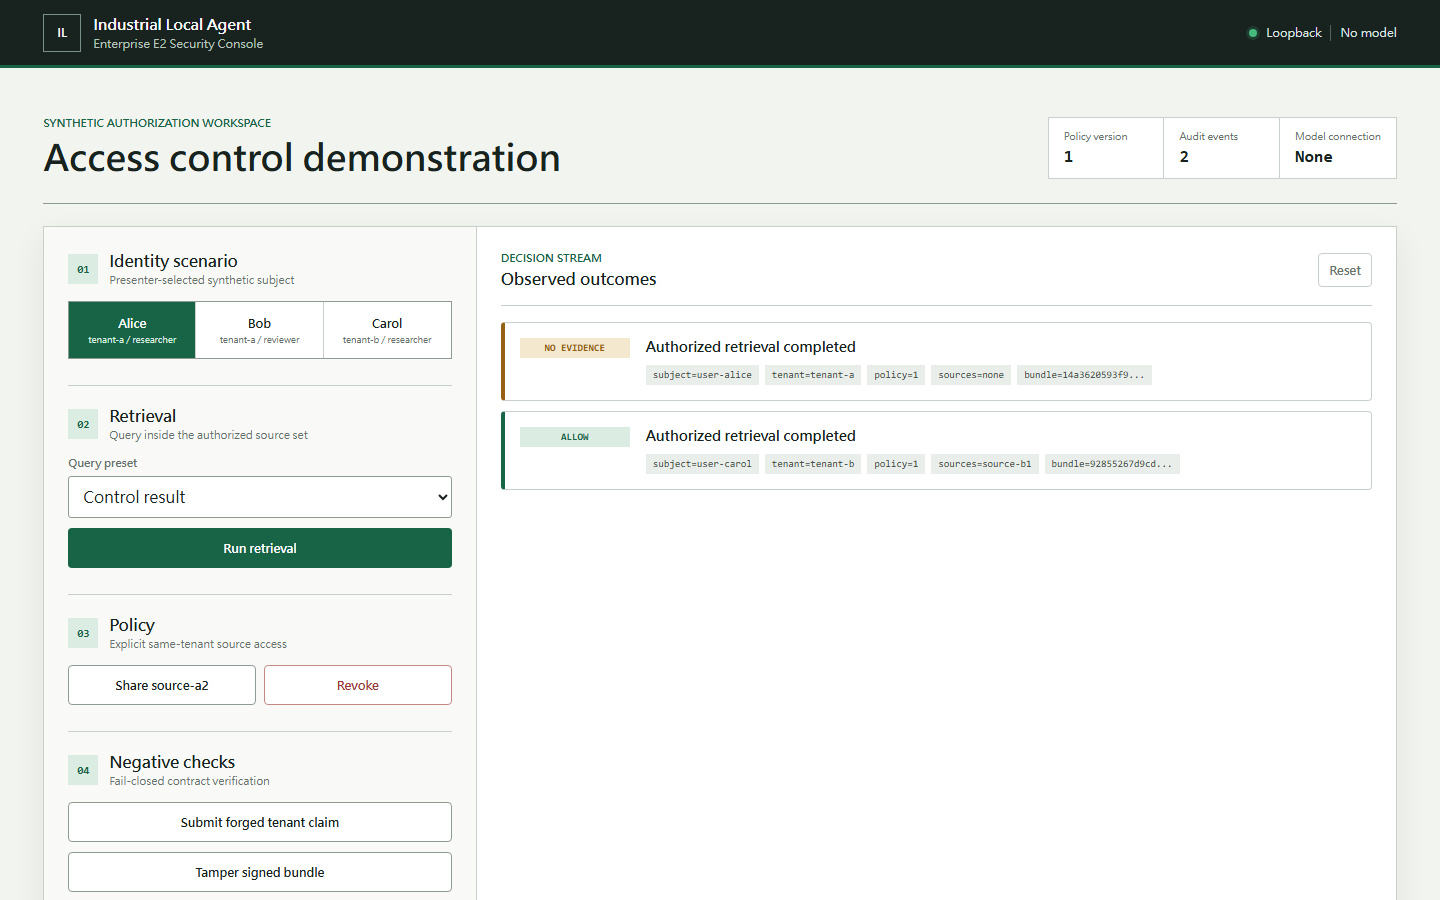
\includegraphics[width=0.86\linewidth,trim=0 150bp 0 0,clip]{assets/demo/e2-tenant-isolation-full.png}%
    }
  \endgroup
\end{uqbody}
\end{frame}

% 6. Live demo: share and revoke
\begin{frame}[plain,t]
\UQFrameHeader{Executed Demo II: Share and Revoke}
\begin{uqbody}
  \vspace{-0.8mm}
  \centering
  \begingroup
    \setlength{\fboxsep}{0pt}
    \setlength{\fboxrule}{0.45pt}
    \fcolorbox{black!32}{white}{%
      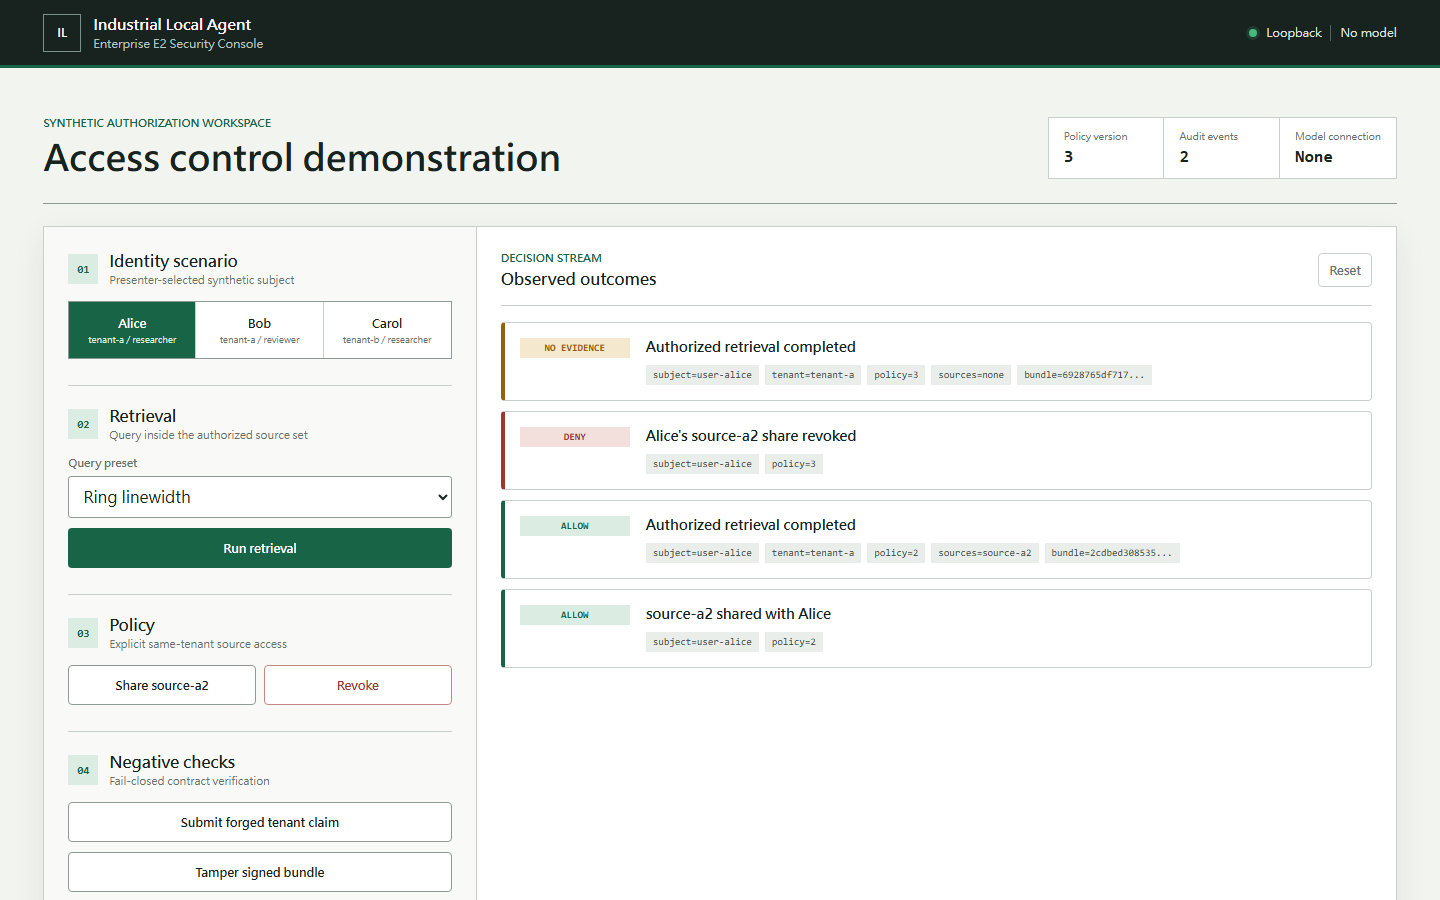
\includegraphics[width=0.86\linewidth,trim=0 150bp 0 0,clip]{assets/demo/e2-share-revoke-full.png}%
    }
  \endgroup
\end{uqbody}
\end{frame}

% 7. Verification evidence and boundary
\begin{frame}[plain,t]
\UQFrameHeader{What the Demo Proves}
\begin{uqbody}
  \UQTakeaway
    {The access contract is testable; the production deployment is the next engineering step.}
    {}

  \vspace{3.1mm}
  \begin{tikzpicture}[x=1cm,y=1cm]
    \node[currentbox,text width=62mm,minimum height=18mm,anchor=north west] at (0,3.75) {%
      {\color{StatusPinned}\fontsize{6.2}{7.3}\selectfont\bfseries TENANT ISOLATION}\par
      Carol: ALLOW\\Alice: NO EVIDENCE
    };
    \node[currentbox,text width=62mm,minimum height=18mm,anchor=north west] at (7.10,3.75) {%
      {\color{StatusPinned}\fontsize{6.2}{7.3}\selectfont\bfseries POLICY LIFECYCLE}\par
      share $\rightarrow$ ALLOW $\rightarrow$ revoke
    };
    \node[currentbox,text width=62mm,minimum height=18mm,anchor=north west] at (0,1.45) {%
      {\color{StatusPinned}\fontsize{6.2}{7.3}\selectfont\bfseries NEGATIVE PATHS}\par
      forged claim, tampered bundle: DENY
    };
    \node[currentbox,text width=62mm,minimum height=18mm,anchor=north west] at (7.10,1.45) {%
      {\color{StatusPinned}\fontsize{6.2}{7.3}\selectfont\bfseries AUDIT CHAIN}\par
      PASS: signed bundle and content-free hash chain
    };
  \end{tikzpicture}

  \vspace{1.8mm}
  \centering
  \UQStatusBadge{StatusPinned}{26 PASSED}
  \hspace{2mm}
  \UQStatusBadge{StatusPinned}{CLI + WEB SHARE ONE RUNTIME}
  \hspace{2mm}
  \UQStatusBadge{StatusDesign}{SYNTHETIC ONLY}

  \vspace{3.4mm}
  {\fontsize{7.2}{8.5}\selectfont
    Next integration: UQ identity, production RLS/RAG, model gateway, and approved compute path.}
\end{uqbody}
\end{frame}

% 8. Hardware and larger-model planning
\begin{frame}[plain,t]
\UQFrameHeader{Bunya Model Plan: Quality vs Cost}
\begin{uqbody}
  \UQTakeaway
    {The LLM is replaceable; Agent contracts stay model-independent.}
    {}

  \vspace{2.5mm}
  \begin{tikzpicture}[x=1cm,y=1cm]
    \node[currentbox,text width=39mm,minimum height=38mm,anchor=north west] at (0,4.05) {%
      {\color{StatusPinned}\fontsize{6.3}{7.4}\selectfont\bfseries LOCAL DEMO}\par\vspace{1.0mm}
      {\fontsize{8.3}{10.0}\selectfont\bfseries 3B model}\par\vspace{1.0mm}
      {\fontsize{7.1}{8.7}\selectfont
        Observed on 12 GB GPU\\
        E2 itself is CPU-only\\
        Lowest cost and fastest iteration}
    };
    \node[targetbox,text width=39mm,minimum height=38mm,anchor=north west] at (4.82,4.05) {%
      {\color{StatusReview}\fontsize{6.3}{7.4}\selectfont\bfseries FIRST BUNYA TEST}\par\vspace{1.0mm}
      {\fontsize{8.3}{10.0}\selectfont\bfseries 14B, 4-bit}\par\vspace{1.0mm}
      {\fontsize{7.1}{8.7}\selectfont
        Roughly 9--12 GB VRAM*\\
        Start with 1 GPU, 8 CPU cores, 32 GB RAM\\
        RCC confirms GPU, quota, and charges}
    };
    \node[targetbox,text width=39mm,minimum height=38mm,anchor=north west] at (9.64,4.05) {%
      {\color{StatusDesign}\fontsize{6.3}{7.4}\selectfont\bfseries ESCALATE ONLY IF NEEDED}\par\vspace{1.0mm}
      {\fontsize{8.3}{10.0}\selectfont\bfseries 32B / 70B-class}\par\vspace{1.0mm}
      {\fontsize{7.1}{8.7}\selectfont
        Roughly 20--24 / 40--48 GB VRAM*\\
        More GPU memory, queue time, and serving cost\\
        Benchmark must justify it}
    };
  \end{tikzpicture}

  \vspace{1.7mm}
  \centering
  {\fontsize{7.2}{8.5}\selectfont\bfseries
    Cost drivers: GPU allocation, job time, storage, and serving complexity.}
  \\[0.6mm]
  {\fontsize{6.7}{8.0}\selectfont
    *Planning estimates only; actual VRAM and RCC pricing require a Bunya benchmark.}
\end{uqbody}
\end{frame}

\end{document}
